%% thesis.tex
%% Copyright 2014 Jean Niklas L'orange
%
% This work may be distributed and/or modified under the
% conditions of the LaTeX Project Public License, either version 1.3
% of this license or (at your option) any later version.
% The latest version of this license is in
%   http://www.latex-project.org/lppl.txt
% and version 1.3 or later is part of all distributions of LaTeX
% version 2005/12/01 or later.
%
% This work has the LPPL maintenance status `maintained'.
% 
% The Current Maintainer of this work is Jean Niklas L'orange.
%
% This work consists of the files Makefile, thesis.tex, config.tex and
% fb/front.tex.

\RequirePackage{fix-cm} %% Patch up incompabilities in fonts
\documentclass[a4paper,12pt,oneside]{article}

%% Project commands
% Some of these can be empty, if so desired
\newcommand{\myName}{My Full Name}
\newcommand{\myShortname}{M. Y. Name}
\newcommand{\myTitle}{My Title}
\newcommand{\myProject}{My Project} %% I usually tend to set this to \myTitle
\newcommand{\myDept}{My Department}
\newcommand{\myFaculty}{My Faculty}
\newcommand{\myUni}{My University}
\newcommand{\myDate}{My Date}
\newcommand{\mySupervisor}{My Supervisor}

%% config.tex
%% Copyright 2014 Jean Niklas L'orange
%
% This work may be distributed and/or modified under the
% conditions of the LaTeX Project Public License, either version 1.3
% of this license or (at your option) any later version.
% The latest version of this license is in
%   http://www.latex-project.org/lppl.txt
% and version 1.3 or later is part of all distributions of LaTeX
% version 2005/12/01 or later.
%
% This work has the LPPL maintenance status `maintained'.
% 
% The Current Maintainer of this work is Jean Niklas L'orange.
%
% This work consists of the files Makefile, thesis.tex, config.tex and
% fb/front.tex.

%% Layout
\usepackage[top=3cm]{geometry}    % Use geometry sizes for margins
\usepackage{mparhack}             % Fix margins
\usepackage[titles]{tocloft}      % For more control of TOC

%% Fix spacing between chapters, sections, subsections
% \setlength{\cftbeforechapskip}{0pt}
\setlength{\cftbeforesecskip}{-10pt}
\setlength{\cftbeforesubsecskip}{-10pt}

%% Fonts and input encoding
\usepackage[utf8]{inputenc}     % Fix input encoding (ish)

% \usepackage{tgpagella}        % TeX Gyre Pagella as main font
% \usepackage[scaled]{beramono} % Correctly scaled (?) Bera Mono as monospace

% Use Bitstream charter as main font
\usepackage[charter, uppercase=upright]{mathdesign}
\usepackage{eulervm}          % Use eulervm for beautiful math fonts
\newcommand{\semibold}{\fontseries{sb}\selectfont}
\usepackage[T1]{fontenc}      % Correct font encoding (T1)
\usepackage{textcomp}         % Fix error messages that fonts are swapped out

%% Header and footer setup

\usepackage{fancyhdr} % Nice-looking headers
\pagestyle{fancy}

%% fancyhdr setup
\fancyfoot{}
\cfoot{}
\fancyhead{}
\fancyhead[RO,LE]{\thepage}
\fancyhead[RE]{\textit{Section \thechapter: \leftmark}}
\fancyhead[LO]{\textit{\rightmark}}

\renewcommand{\sectionmark}[1]{\markboth{#1}{}}
\renewcommand{\subsectionmark}[1]{\markright{\thesubsection\quad#1}{}}
\setlength{\headheight}{15pt}

%% Citation and Bibliography selections.
\usepackage[citestyle=numeric,bibstyle=numeric,firstinits=true,backend=biber,%
  maxcitenames=2,mincitenames=1,maxbibnames=20,minbibnames=20,sorting=none,%
  urldate=long]{biblatex}

%% For a more visually pleasing layout (comment to save space)
\setlength{\parskip}{\bigskipamount}
\setlength{\parindent}{0pt}

%% Misc. packages
\usepackage{tabularx}                    % Better tabular
\usepackage{caption}                     % Better captions
\usepackage{chngcntr}                    % Change counter for listings
\usepackage{subcaption}                  % Add subcaptions
\usepackage{wrapfig}                     % Add wrapfigs
\usepackage{color}                       % Add in color (by name)
\usepackage[usenames,dvipsnames]{xcolor} % Many more color names here

\captionsetup{
  figurewithin=section,
  tablewithin=section
}

%% Links in the PDF
\definecolor{webgreen}{rgb}{0,.5,0} % Web green
\definecolor{webbrown}{rgb}{.6,0,0} % Web brown
\definecolor{solarizedblue}{HTML}{268BD2}

\newcommand{\cvar}[1]{\textit{#1}}

\usepackage{hyperref}
\hypersetup{
    %draft, % Smart to add so that one avoids sending the wrong PDF :). Tick off
            % when sending the real deal.
    colorlinks=true, linktocpage=true, pdfstartpage=1, pdfstartview=FitV,
    breaklinks=true, pdfpagemode=UseNone, pageanchor=true,
    pdfpagemode=UseOutlines,plainpages=false, bookmarksnumbered,
    bookmarksopen=true, bookmarksopenlevel=1, hypertexnames=true,
    pdfhighlight=/O,
    urlcolor=webbrown, linkcolor=RoyalBlue, citecolor=webgreen,
    pdftitle={\myTitle},
    pdfauthor={\textcopyright\ \myShortname, \myUni, \myDept},
    pdfsubject={\myProject},
}

%% Listing packages

%%% NB: REQUIRES pygments (python-pygments) installed to work.
\usepackage[section]{minted}        % Minted, good pygments wrapper
\usemintedstyle{colorful}           % Mintedstyle

\usepackage{algpseudocode}
\algrenewcommand\alglinenumber[1]{\scriptsize #1\quad}

% define ruled float, but with naming at bottom. Used for algorithms in
% listings.
\makeatletter
\newcommand\fs@plainruled{\def\@fs@cfont{\rmfamily}\let\@fs@capt\floatc@plain%
  \def\@fs@pre{\hrule\kern2pt}%
  \def\@fs@mid{\kern2pt\hrule\vspace\abovecaptionskip\relax}%
  \def\@fs@post{}%
  \let\@fs@iftopcapt\iffalse}

\newcommand\floatc@bottomruled[2]{{\@fs@cfont #1} #2\par}
\newcommand\fs@bottomruled{\def\@fs@cfont{\bfseries}\let\@fs@capt\floatc@bottomruled
  \def\@fs@pre{\hrule height.8pt depth0pt \kern2pt}%
  \def\@fs@post{\kern2pt\hrule\relax}%
  \def\@fs@mid{\kern2pt\hrule\kern2pt}%
  \let\@fs@iftopcapt\iffalse}
\makeatother

%% New environment for algorithms
\newenvironment{alglisting}[1][ht]
  {\floatstyle{plainruled}%
\restylefloat{listing}%
   \begin{listing}[#1]
  }{\end{listing}}
\counterwithin{listing}{section}

%% Math packages
\usepackage{amsmath}          % Symbols, math modes, etc.
\usepackage{mathtools}        % Typesetting and fix bugs in amssymb
\usepackage{amsthm}           % For theorems

\usepackage{xspace}   % Fix space between macros.
\usepackage{fixltx2e} % General fix on misc. other fails

%% Setting up chapter
\usepackage{titlesec}
\titlespacing\section{0pt}{0pt plus 4pt minus 2pt}{0pt plus 2pt minus 2pt}

\titleformat{\chapter}[display]
{\normalfont\filcenter\semibold}
{\sc{\Large \chaptertitlename\ \thechapter}}
{0pt}
{\LARGE}

%% By default, add fig/ as a place to look for graphics.
\usepackage{graphicx}
\graphicspath{{fig/}}

%% Add in \TODO command, for inline TODOS.
\newcommand{\TODO}[1]{\textcolor{red}{\textbf{TODO:} #1}}

%% Add in \O command, for use within math environments
\renewcommand{\O}{\mathcal{O}}


% Package lipsum for dummy text. No need to keep it unless you actually need
% dummy text.
\usepackage{lipsum}

%% Bibliography resources. You can add more if you like to have them separated
%% in different files.
\addbibresource{bib/bibliography.bib}

\begin{document}
\frenchspacing
\raggedbottom

%% fb/front.tex
%% Copyright 2014 Jean Niklas L'orange
%
% This work may be distributed and/or modified under the
% conditions of the LaTeX Project Public License, either version 1.3
% of this license or (at your option) any later version.
% The latest version of this license is in
%   http://www.latex-project.org/lppl.txt
% and version 1.3 or later is part of all distributions of LaTeX
% version 2005/12/01 or later.
%
% This work has the LPPL maintenance status `maintained'.
% 
% The Current Maintainer of this work is Jean Niklas L'orange.
%
% This work consists of the files Makefile, thesis.tex, config.tex and
% fb/front.tex.

%% Opening page
\thispagestyle{empty}
\addtocounter{page}{-1}

\begin{center}
  \LARGE {\semibold \myProject}

  \vfill

  %% Front page grahics, if you like
  \begin{figure}[h]
    \centering
    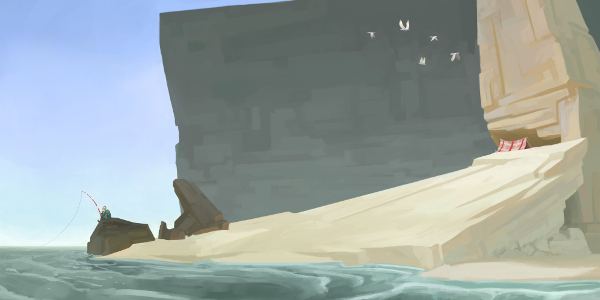
\includegraphics[width=8cm]{rock}
  \end{figure}

  \vfill
  \large A master dissertation presented by
  \vspace{5mm}

  {\semibold \myName}

  \vspace{5mm}

  in partial fulfillment of the requirements for the degree of Master of
  Science.

  \vfill

  Supervisor: \mySupervisor

  \vfill
  \myDept \\
  \myUni \\
  \myDate
\end{center}
\skiponepage


%% Abstract and acknowledgements
\thispagestyle{plain}
\pagenumbering{alph}
%% Template for abstract.tex.
%% Not under the license, just here to ensure the template compiles properly.

\chapter*{Abstract}
\addcontentsline{toc}{chapter}{Abstract}

Here will my abstract be.


\pagenumbering{arabic}
\pagestyle{fancy}

%% Here you insert chapters as you go
%% Dummy intro.tex.
%% Not under the license, just here to ensure the template compiles properly.
%% Also contains a couple of examples.

\section{Introduction}\label{sec:intro}

\subsection{Examples}

\lipsum[1-2]

\begin{equation} \label{eq:heart-eq}
  F\left\{ \heartsuit \right \} =
  \frac{1}{\sqrt{2\pi}} \int\limits_{-\infty}^{\infty} f(t) e^{i t \heartsuit} \mathrm{d} t
  = \text{\textbf{?}}
\end{equation}

Equation (\ref{eq:heart-eq}) shows us that this is still an unsolved problem.

\lipsum[3]

\begin{figure}
  \centering
  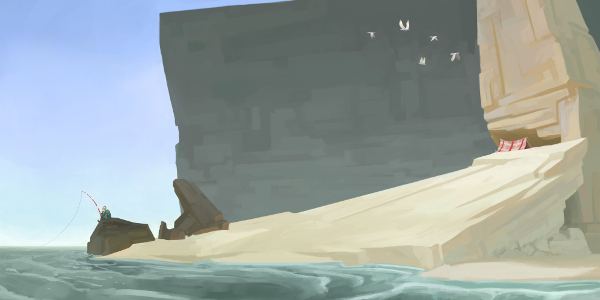
\includegraphics[width=0.8\linewidth]{rock}
  \caption[Rock]{\emph{Rock} by David Smit, licensed under a \emph{Creative
      Commons Attribution-NonCommercial 3.0 Unported License}.}
  \label{fig:rock}
\end{figure}

Figure \ref{fig:rock} is the same figure as the front page figure. The
difference is that we use it to give an example on how to center and include it
as a figure.

\lipsum[4]

Citation of the C11 standard\cite{iso2011c}.

\lipsum[11-12]

\begin{listing}
  \inputminted[frame=single,linenos,fontsize=\small,mathescape]{scm}{lst/sqrt-iter.scm}
  \caption[Square Roots in Scheme]{Implementation of Square Roots by Newton's
    Method in Scheme, from SICP.}
  \label{lst:sqrt-iter}
\end{listing}

Listing \ref{lst:sqrt-iter} shows us how code blocks will look like. Change the
colours palette inside \texttt{config.tex} if you want another one.

\begin{alglisting}
  \begin{algorithmic}[1]
    \Function{\texttt{floyd-warshall}}{$E$}
    \State $N \gets$ \Call{len}{$P$}
    \State $next \gets $ \Call{int-array}{$N$, $N$}
    \For{$i \gets 0$ \textbf{below} $N$} \Comment{Populate with infinite edges}
      \For{$j \gets 0$ \textbf{below} $N$}
        \State $next[i][j] \gets \infty$
      \EndFor
    \EndFor
    \For{$k \gets 0$ \textbf{below} $N$}
      \For{$i \gets 0$ \textbf{below} $N$}
        \For{$j \gets 0$ \textbf{below} $N$}
          \If{$E[i][k] + E[k][j] < E[i][j]$}
            \State $E[i][j] \gets E[i][k] + E[k][j]$
            \State $next[i][j] \gets k$
          \EndIf
        \EndFor
      \EndFor
    \EndFor
    \State \Return $E$ \Comment{Or the next matrix if you want}
    \EndFunction
  \end{algorithmic}
  \caption{Implementation of \textsc{\texttt{floyd-warshall}}.}
  \label{lst:floyd-warshall}
\end{alglisting}


Floyd-Warshall is presented in \ref{lst:floyd-warshall}. I personally prefer the
looks in Tethys Thesis for alglistings, as the font in that template has
smallcaps -- Quattrocento doesn't.

\lipsum[13]


\printbibliography

\end{document}
